
\subsection*{Part 1}

\begin{align*}
    u = 0.05 \implies f(\theta) = s\frac{1-u}{u} = 0.36\\
\end{align*}

\begin{align*}
    f(\theta) &= M(1, \theta) = \frac{\theta}{(1+\theta^\iota)^{1/\iota}}\\
    \implies \theta = 0.4123
\end{align*}

Hence $\theta = 0.4123$ is consistent with $u = 0.05$.\\

From the free entry and wage condition in steady state
\begin{align*}
    c &= \beta q(\theta) \frac{1}{1 - \beta(1 - s)} [(1 - \gamma)(z - b) - \gamma \theta c]\\
    \implies c &= 1.288
\end{align*}


\subsection*{Part 2}
Transition matrix is given by

\begin{equation*}
    P = \begin{bmatrix}
        \pi~, 1-\pi \\
        1- \pi~~~, \pi
    \end{bmatrix}
\end{equation*}

It has a unique stationary state 
\begin{align*}
    p = \begin{bmatrix}
        0.5 \\ 
        0.5
    \end{bmatrix}
\end{align*}

Since $\mathbb E[\log z] = 0$ and $Var[\log z] = 0.0001$, we have 
\begin{align*}
    \log z_h &= -\log z_l\\
    (\log z_h)^2 + (\log z_l)^2 &= 2*0.0001
\end{align*}

which gives 
$$ z_h = e^{0.01}~~~,~~~ z_l = e^{-0.01}$$

The autocorrelation is 
\begin{align*}
    \rho &= \frac{\mathbb{E}[\log z_t \log z_{t+1}]}{\operatorname{Var}(\log z_t)} \\
    &= \frac{\mathbb{E}\left[ \log z_t \mathbb{E}[\log z_{t+1} \mid \log z_t] \right]}{\operatorname{Var}(\log z_t)}
\end{align*}

Substituting $\mathbb{E}[\log z_{t+1} \mid \log z_t] = \pi \log z_t - (1-\pi)\log z_t$ gives
\begin{align*}
    \rho = 2\pi - 1 \implies \pi = 0.985
\end{align*}

\subsection*{Part 3}

Free entry condition and value of filling a position is 
\begin{align*}
c &= \beta q(\theta(z,u)) \mathbb{E}_{z',u'} [J(z',u')|z] \\
J(z,u) &= z - w(z,u) + \beta(1-s) \mathbb{E}_{z',u'} [J(z',u')|z] \\
\end{align*}
where $w(z,u) = (1-\gamma)b + \gamma(z + \theta(z,u)c)$.\\

$\theta(z, u)$ and $J(z, u)$ do not depend on u, so that we can write $\theta(z)$ and $J(z)$. WHY?\\

We have
\begin{align*}
    q(\theta) = M(1/\theta, 1) =  \frac{1}{(1+\theta^\iota)^{1/\iota}}   
\end{align*}

The 4 equations in terms of $\{\theta(z_l ), \theta(z_h), J(z_l ), J(z_h)\}$ are

\begin{align*}
    \frac{c}{\beta } (1+\theta(z_h)^\iota)^\frac{1}{\iota} &= \pi J(z_h) + (1-\pi) J(z_l) \\
    \frac{c}{\beta } (1+\theta(z_l)^\iota)^\frac{1}{\iota} &= \pi J(z_l) + (1-\pi) J(z_h) \\
    J(z_h) &= (1-\gamma)(z_h - b) - \gamma c \theta(z_h) + \beta (1-s)[\pi J(z_h) + (1-\pi) J(z_l)]\\
    J(z_l) &= (1-\gamma)(z_l - b) - \gamma c \theta(z_l) + \beta (1-s)[\pi J(z_l) + (1-\pi) J(z_h)]\\    
\end{align*}

Solving these gives
\begin{align*}
    \theta(z_h) &= 0.419631 \\
    \theta(z_l) &= 0.404967 \\
    J(z_h) & = 1.485272 \\
    J(z_l) & = 1.474688 \\
\end{align*}


The simulation results are in figure \ref{fig:q3_sim_b0.4}. The standard deviations are
\begin{align*}
    sd(\log z_t) &= 0.010\\
    sd(\log u_t) &= 0.013\\
    sd(\log v_t) &= 0.007\\
    sd(\log \theta_t) &= 0.018\\    
\end{align*}

\begin{figure}[H]
    \centering
    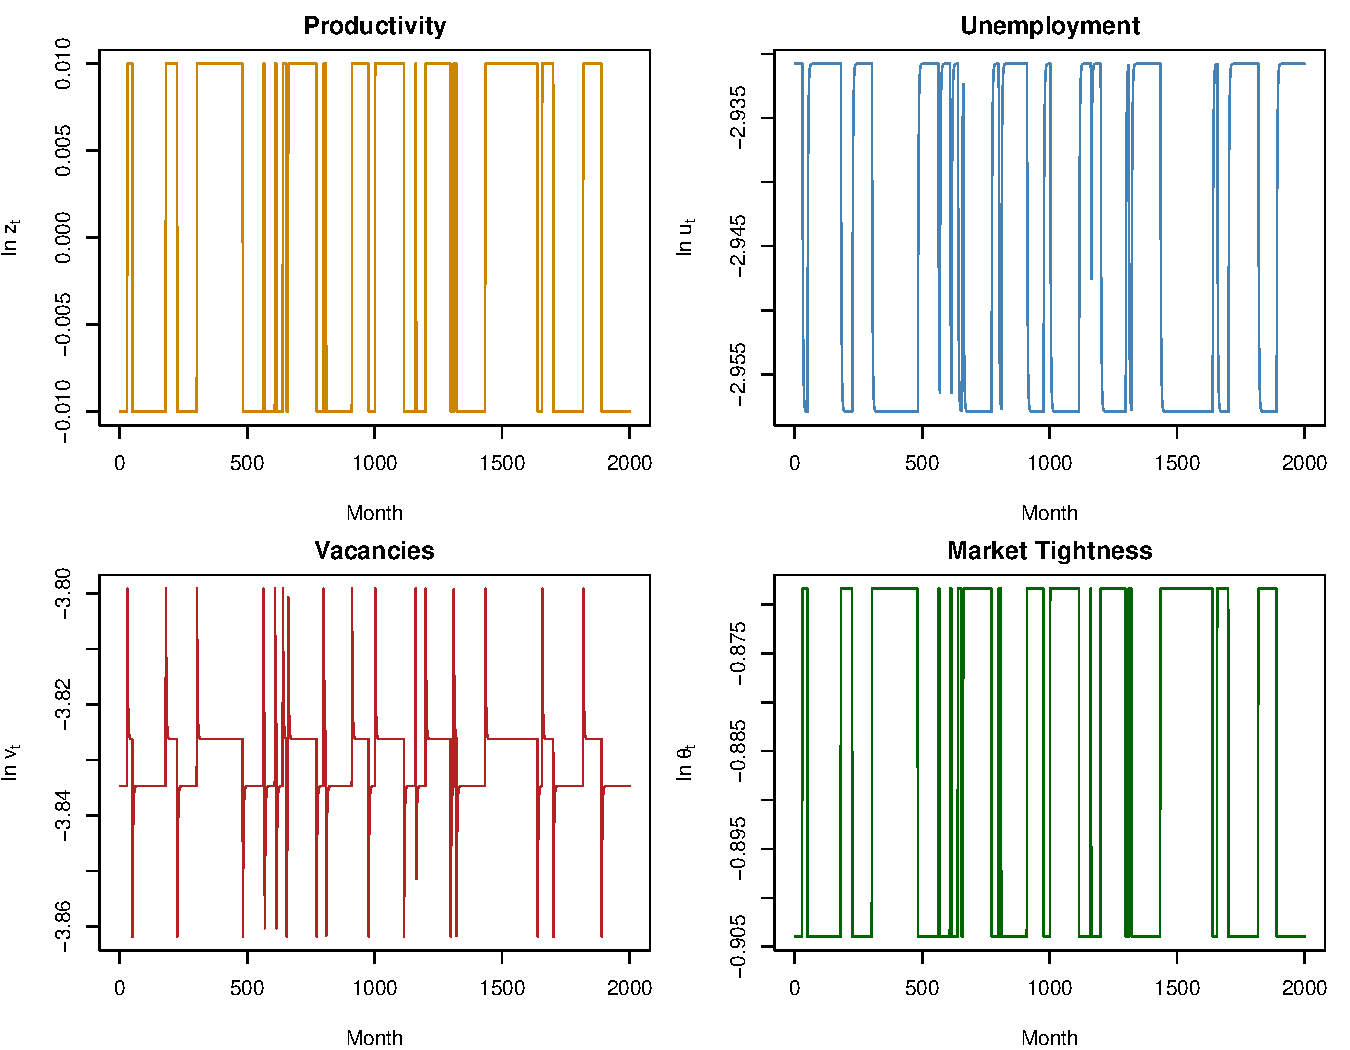
\includegraphics[width=1\textwidth]{Figures/plot_q3_part3_sim_b_0.4.pdf}
    \caption{Simulation Results for $b=0.4$}
    \label{fig:q3_sim_b0.4}
\end{figure}

\subsection*{Part 4}
With $b = 0.96$, we have the new params

\begin{align*}
    c &=  0.1073\\
    \theta(z_h) &= 0.500729 \\
    \theta(z_l) &= 0.324690 \\
    J(z_h) & = 0.128870 \\
    J(z_l) & = 0.118311 \\
\end{align*}

the simulation results are in figure \ref{fig:q3_sim_b0.95}. The standard deviations are 
\begin{align*}
    sd(\log z_t) &= 0.010\\
    sd(\log u_t) &= 0.160\\
    sd(\log v_t) &= 0.082\\
    sd(\log \theta_t) &= 0.217\\    
\end{align*}


\begin{figure}[H]
    \centering
    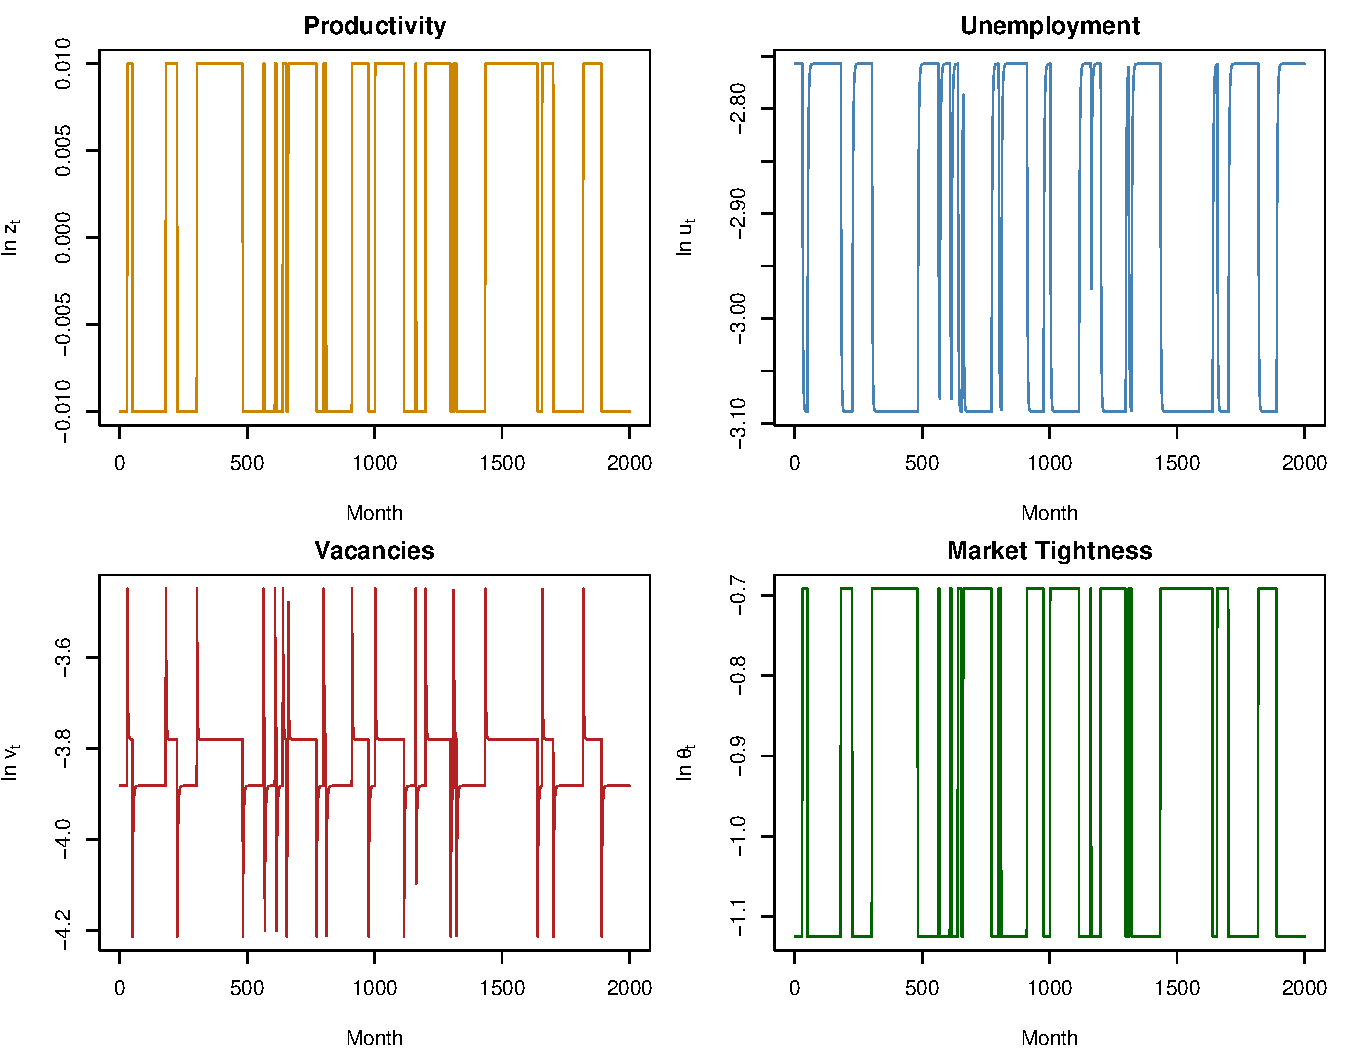
\includegraphics[width=1\textwidth]{Figures/plot_q3_part3_sim_b_0.95.pdf}
    \caption{Simulation Results for $b=0.95$}
    \label{fig:q3_sim_b0.95}
\end{figure}


\subsection*{Part 5}
Let flow utility be $b= \bar b z_t$. Then the 4 equations are 

\begin{align*}
    \frac{c}{\beta } (1+\theta(z_h)^\iota)^\frac{1}{\iota} &= \pi J(z_h) + (1-\pi) J(z_l) \\
    \frac{c}{\beta } (1+\theta(z_l)^\iota)^\frac{1}{\iota} &= \pi J(z_l) + (1-\pi) J(z_h) \\
    J(z_h) &= (1-\gamma)(1 - \bar b)z_h - \gamma c \theta(z_h) + \beta (1-s)[\pi J(z_h) + (1-\pi) J(z_l)]\\
    J(z_l) &= (1-\gamma)(1 - \bar b)z_l - \gamma c \theta(z_l) + \beta (1-s)[\pi J(z_l) + (1-\pi) J(z_h)]\\    
\end{align*}

which gives the solutions
\begin{align*}
    c &=  0.1073\\
    \theta(z_h) &= 0.416790 \\
    \theta(z_l) &= 0.407990 \\
\end{align*}


the simulation results are in figure \ref{fig:q3_sim_part5}. The standard deviations are 
\begin{align*}
    sd(\log z_t) &= 0.010\\
    sd(\log u_t) &= 0.008\\
    sd(\log v_t) &= 0.004\\
    sd(\log \theta_t) &= 0.011\\    
\end{align*}

\begin{figure}[H]
    \centering
    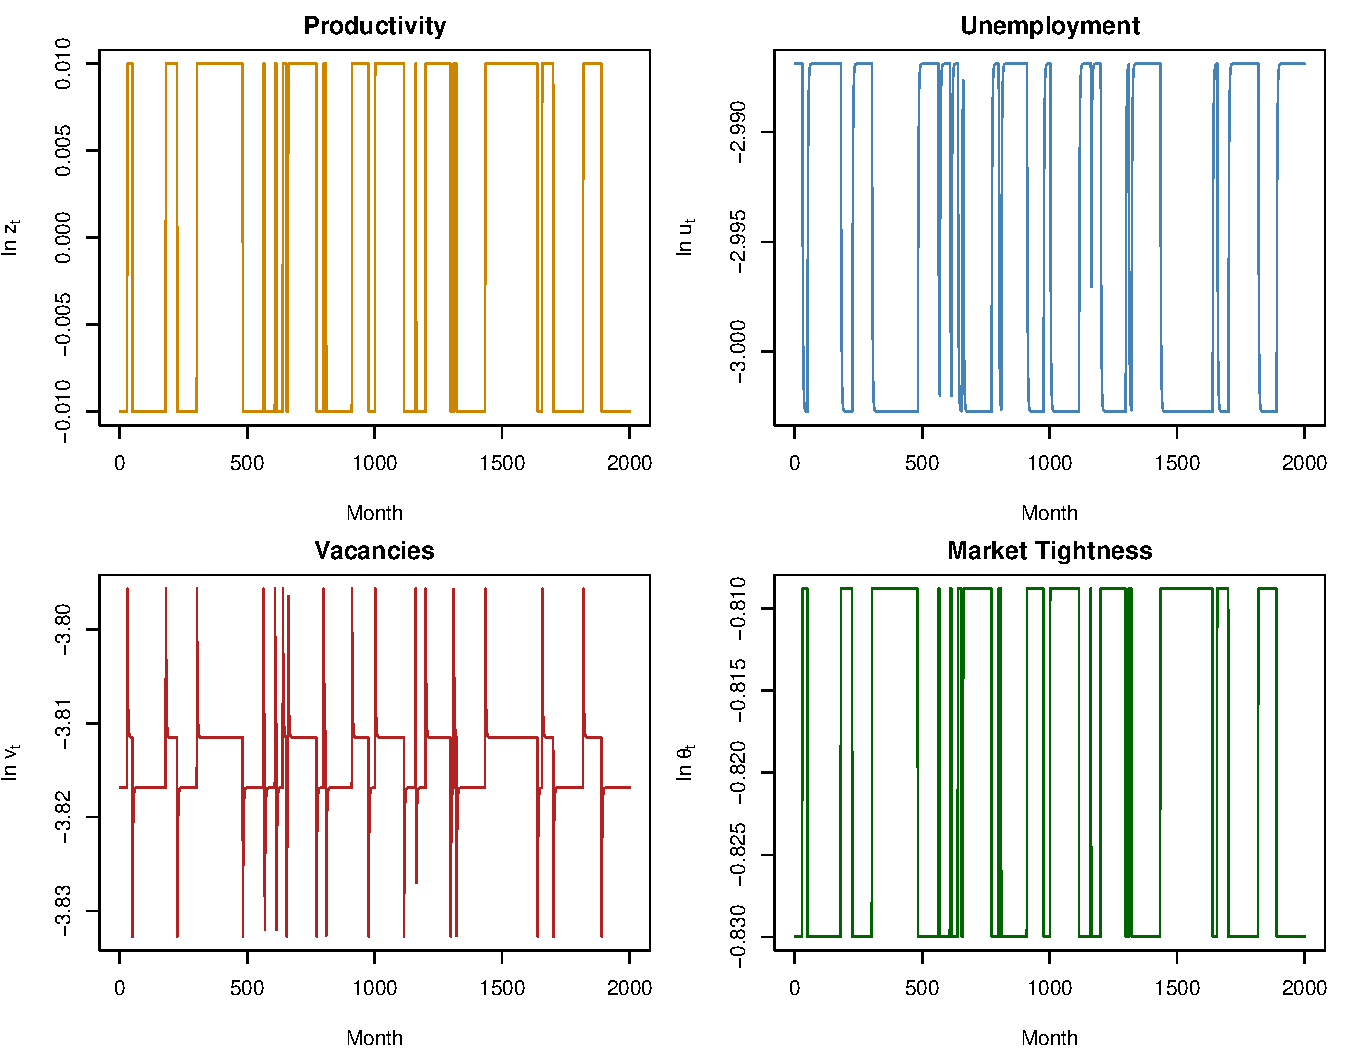
\includegraphics[width=1\textwidth]{Figures/plot_q3_part5_sim.pdf}
    \caption{Simulation Results for $b_t=0.95\times z_t$}
    \label{fig:q3_sim_part5}
\end{figure}



\subsection*{Part 6}
Let rigid wages be $w_t = \bar w = 0.95$. Then the 4 equations are 

\begin{align*}
    \frac{c}{\beta } (1+\theta(z_h)^\iota)^\frac{1}{\iota} &= \pi J(z_h) + (1-\pi) J(z_l) \\
    \frac{c}{\beta } (1+\theta(z_l)^\iota)^\frac{1}{\iota} &= \pi J(z_l) + (1-\pi) J(z_h) \\
    J(z_h) &= z_h - \bar w + \beta (1-s)[\pi J(z_h) + (1-\pi) J(z_l)]\\
    J(z_l) &= z_l - \bar w + \beta (1-s)[\pi J(z_l) + (1-\pi) J(z_h)]\\    
\end{align*}

which gives the solutions
\begin{align*}
    c &=  0.1073\\
    \theta(z_h) &= 21.540219 \\
    \theta(z_l) &= 18.105566 \\
\end{align*}


the simulation results are in figure \ref{fig:q3_sim_part6}. The standard deviations are 
\begin{align*}
    sd(\log z_t) &= 0.010\\
    sd(\log u_t) &= 0.0007\\
    sd(\log v_t) &= 0.086\\
    sd(\log \theta_t) &= 0.087\\    
\end{align*}

\begin{figure}[H]
    \centering
    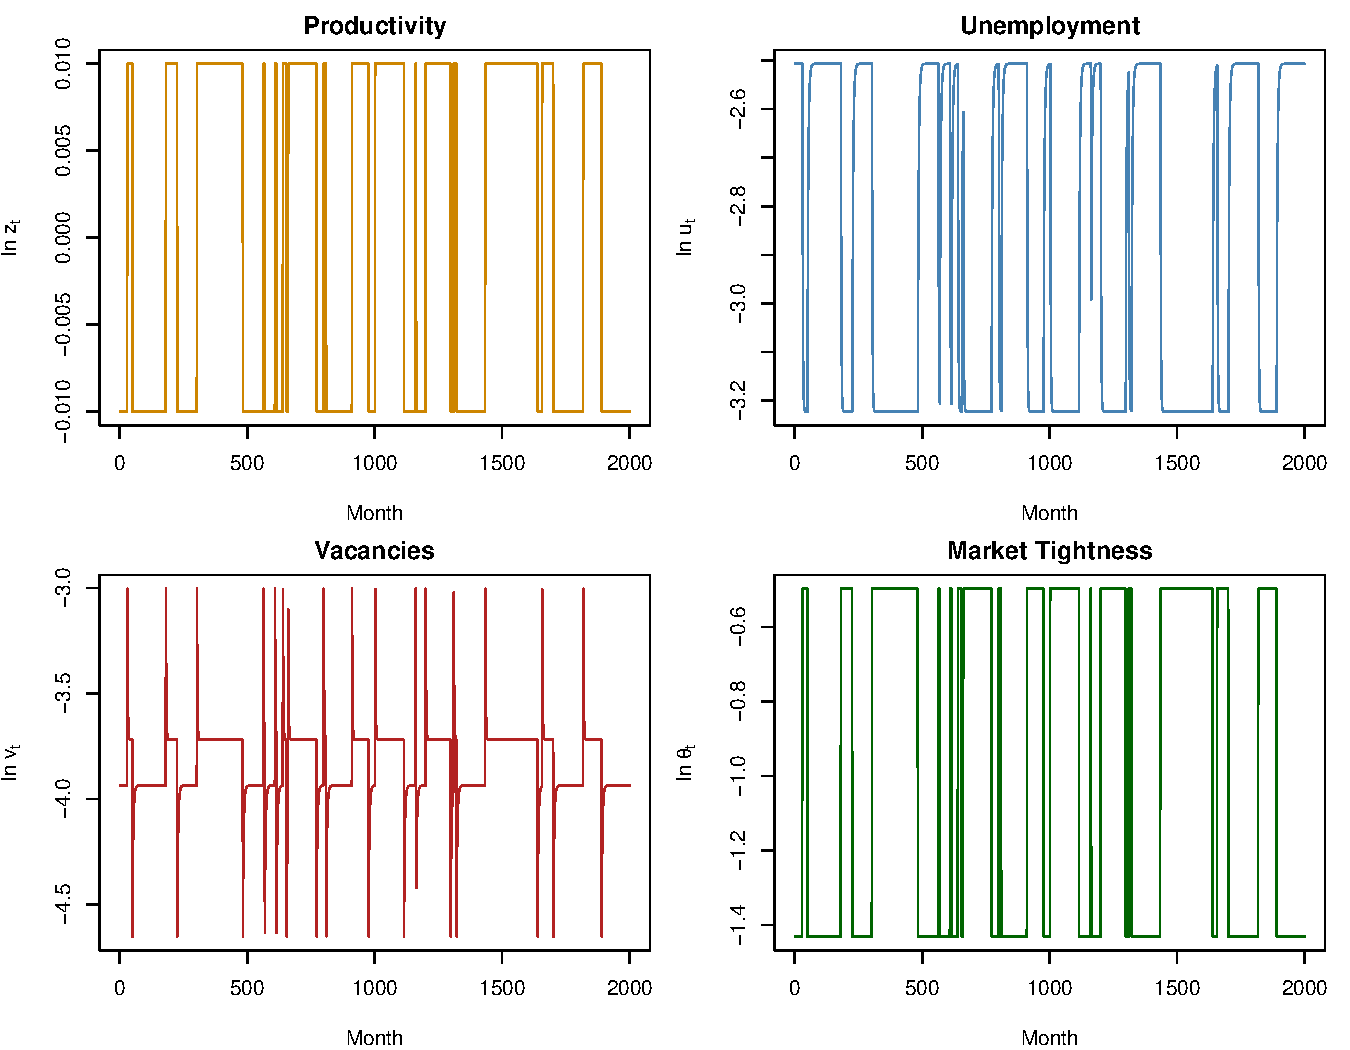
\includegraphics[width=1\textwidth]{Figures/plot_q3_part6_sim.pdf}
    \caption{Simulation Results for $w_t=\bar w = 0.95$}
    \label{fig:q3_sim_part6}
\end{figure}